% Figure: the continuous four-stage cycle (S1 passive monitor, S2 triage and alert, S3 approved
% pentest over SSH under ROE, S4 dual reporting), its actors and trust boundaries, and the
% adversaries A1..A7. The dashed box (external pentest toolkit) is optional.
% Build: pdflatex architecture.tex -> architecture.pdf (included by ../paper.tex)
\documentclass[tikz,border=2pt]{standalone}
\usepackage[T1]{fontenc}
\usepackage[utf8]{inputenc}
\usepackage{helvet}
\renewcommand{\familydefault}{\sfdefault}
\usetikzlibrary{fit,arrows.meta,backgrounds,calc}
\begin{document}
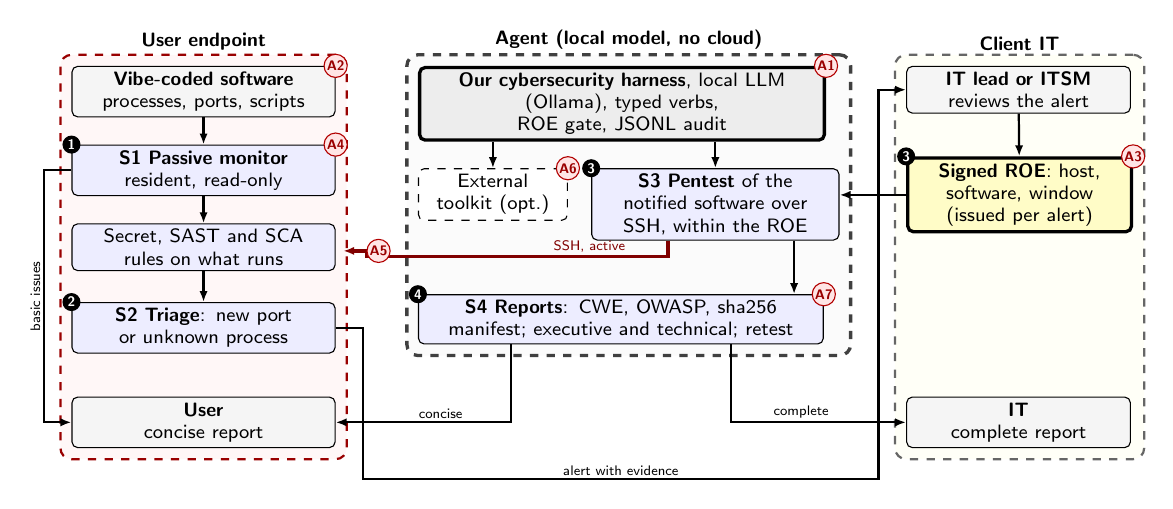
\begin{tikzpicture}[
  font=\sffamily\scriptsize,
  box/.style={draw, rounded corners=2pt, fill=white, align=center, inner sep=2pt, anchor=north west},
  impl/.style={box, fill=blue!7},
  stg/.style={circle, draw, fill=black, text=white, inner sep=0.6pt, font=\sffamily\tiny\bfseries},
  arr/.style={-{Latex[length=1.4mm]}, thick},
  adv/.style={circle, draw=red!70!black, fill=red!10, text=red!60!black, inner sep=0.4pt, font=\sffamily\tiny\bfseries},
  lbl/.style={font=\sffamily\tiny, inner sep=1pt, align=center},
]
% ---------------- user endpoint ----------------
\node[box, text width=3.2cm, fill=gray!8] (sw) at (0,6.6) {\textbf{Vibe-coded software}\\processes, ports, scripts};
\node[impl, text width=3.2cm] (s1) at (0,5.6) {\textbf{S1 Passive monitor}\\resident, read-only};
\node[impl, text width=3.2cm] (rules) at (0,4.6) {Secret, SAST and SCA\\rules on what runs};
\node[impl, text width=3.2cm] (s2) at (0,3.6) {\textbf{S2 Triage}: new port\\or unknown process};
\node[box, text width=3.2cm, fill=gray!8] (user) at (0,2.4) {\textbf{User}\\concise report};
\draw[arr] (sw) -- (s1);
\draw[arr] (s1) -- (rules);
\draw[arr] (rules) -- (s2);
\begin{scope}[on background layer]
\node[draw=red!60!black, dashed, thick, rounded corners=4pt, inner sep=4pt, fill=red!3, fit=(sw)(s1)(rules)(s2)(user)] (ep) {};
\end{scope}
\node[anchor=south, font=\sffamily\scriptsize\bfseries, inner sep=1pt] at (ep.north) {User endpoint};
\draw[arr] (s1.west) -- ++(-0.35,0) |- node[pos=0.25, lbl, rotate=90, above]{basic issues} (user.west);

% ---------------- agent ----------------
\node[box, text width=5.0cm, fill=gray!14, very thick] (eng) at (4.4,6.6) {\textbf{Our cybersecurity harness}, local LLM\\(Ollama), typed verbs, ROE gate, JSONL audit};
\node[box, text width=1.75cm, dashed] (har) at (4.4,5.3) {External\\toolkit (opt.)};
\node[impl, text width=3.0cm] (s3) at (6.6,5.3) {\textbf{S3 Pentest} of the\\notified software over\\SSH, within the ROE};
\node[impl, text width=5.0cm] (s4) at (4.4,3.7) {\textbf{S4 Reports}: CWE, OWASP, sha256\\manifest; executive and technical; retest};
\draw[arr] (eng.south-|har.north) -- (har);
\draw[arr] (eng.south-|s3.north) -- (s3);
\draw[arr] ([xshift=1.0cm]s3.south) -- ([xshift=1.0cm]s3.south|-s4.north);
\begin{scope}[on background layer]
\node[draw=black!75, dashed, very thick, rounded corners=4pt, inner sep=4pt, fill=gray!3, fit=(eng)(har)(s3)(s4)] (ag) {};
\end{scope}
\node[anchor=south, font=\sffamily\scriptsize\bfseries, inner sep=1pt] at (ag.north) {Agent (local model, no cloud)};

% ---------------- IT ----------------
\node[box, text width=2.7cm, fill=gray!8] (it) at (10.6,6.6) {\textbf{IT lead or ITSM}\\reviews the alert};
\node[box, text width=2.7cm, fill=yellow!22, very thick] (roe) at (10.6,5.45) {\textbf{Signed ROE}: host,\\software, window\\(issued per alert)};
\node[box, text width=2.7cm, fill=gray!8] (itrep) at (10.6,2.4) {\textbf{IT}\\complete report};
\draw[arr] (it) -- (roe);
\begin{scope}[on background layer]
\node[draw=black!60, dashed, thick, rounded corners=4pt, inner sep=4pt, fill=yellow!3, fit=(it)(roe)(itrep)] (itb) {};
\end{scope}
\node[anchor=south, font=\sffamily\scriptsize\bfseries, inner sep=1pt] at (itb.north) {Client IT};

% ---------------- cycle ----------------
\draw[arr] (s2.east) -- ++(0.35,0) |- node[pos=0.75, lbl, above]{alert with evidence} (10.25,1.35) |- (it.west);
\draw[arr] (roe.west) -- (roe.west-|s3.east);
\draw[arr, very thick, red!50!black] (s3.south) ++(-0.6,0) -- ++(0,-0.2) -| node[pos=0.0, above, lbl, text=red!50!black, xshift=-1.0cm]{SSH, active} (3.75,4.25) -- (3.45,4.25);
\draw[arr] ([xshift=-1.4cm]s4.south) |- node[pos=0.7, above, lbl]{concise} (user.east);
\draw[arr] ([xshift=1.4cm]s4.south) |- node[pos=0.7, above, lbl]{complete} (itrep.west);

% ---------------- stage markers ----------------
\node[stg] at (s1.north west) {1};
\node[stg] at (s2.north west) {2};
\node[stg] at (roe.north west) {3};
\node[stg] at (s3.north west) {3};
\node[stg] at (s4.north west) {4};

% ---------------- adversaries ----------------
\node[adv] at (eng.north east) {A1};
\node[adv] at (sw.north east) {A2};
\node[adv] at (roe.north east) {A3};
\node[adv] at (s1.north east) {A4};
\node[adv] at (3.9,4.25) {A5};
\node[adv] at (har.north east) {A6};
\node[adv] at (s4.north east) {A7};
\end{tikzpicture}
\end{document}
